%
% idee.tex -- Polynom Idee
%
\section{Idee
\label{reedsolomon:section:idee}}
\rhead{Problemstellung}
Um Fehler in einer Datenübertragung zu erkennen, könnte man die Daten jeweils doppelt senden,
also den gleichen Wert immer zweimal. 
Tritt ein Fehler ein, wird sich dies in der Differenz der beiden Werte bemerkbar machen.
Aber wie erkennen wir, welcher nun der richtige ist? Die Lösung ist simpel: Wir übertragen den Wert einfach dreimal.
Wenn jetzt ein Fehler auftritt, kann durch die beiden unveränderten Werte der richtige bestimmt werden.
Doch was machen wir, wenn bei dieser Übertragung zwei Fehler auftreten? 
Oder noch schlimmer: Was ist, wenn zweimal derselbe Fehler auftritt? Die beiden fehlerhaften Werte überstimmen bei der Evaluierung den gesendeten Datenwert, der dann unwiderruflich verloren geht. 
Wir könnten dies noch steigern mit vier, fünf oder mehr gleichen übertragenen Werte. Dies erhöht zwar die Robustheit der gesendeten Daten, führt aber auch dazu, dass wir durch die Mehrfachübertragung nur sehr wenige Nutzdaten versenden können.
Gerade in der heutigen Zeit wäre dies ein enorm grosses Problem und aus diesem Grund wurden alternative Ansätze ausgearbeitet, um dieses grundlegende Problem zu lösen. 
%
%
%Gerade in der heutigen modernen Zeit bei dem hohen bedarf an Daten würden unsere Kommunikationssysteme bei weitem nicht ausreichen um den einen einzigen Datenwert mehrfach zu übertragen
%
% Gerade in der Heutigen modernen Zeit bei diesem enormen mass an daten die wir alle tagtäglich anfordern Währe dies wohl unmöglich, wenn wir die daten auf diese Weise 
%
%
%
%
%
%Wenn es uns gelingt, Fehler nach Ihrer Übertragung zu erkennen, dann könnten wir in einem neuen Ansatz den fehlerhaft empfangenen Wert noch einmal anfordern. 
%Wir stellen fest, dass für viele alltägliche Anwendungen völlig ausreichend ist.
%
%Was ist, wenn wir aber eine Datenquelle haben, von der wir nur einmalig lesen können?
%
% 
%
%Beim Übertragen von drei Werten können wir maximal 2 Fehler erkennen aber nicht mehr korrigieren.
%Wenn wir noch mehr Werte 
%
%Wir Übertragen Ziemlich viele Werte für so wenige Nutzdaten. Hinzu kommt, dass wir bei dieser Vorgehensweise gerade mal bestimmen können, dass überhaupt Fehler aufgetreten sind 
%
%
%Wir haben also drei Werte die bestimmt einen Fehler korrigieren können, was ziemlich viele Werte um einen Fehler zu korrigieren. 
%
% um so jeweils einzelne Fehler zu erkennen.
%Wenn jedoch mehr als nur ein Fehler erkannt werden und sogar noch das Original rekonstruiert werden soll, dann sollen die Daten drei oder vierfach versendet werden.
%Doch nur schon um einen Fehler zu erkennen werden überproportional viele Daten doppelt und dreifach versendet.
%Das Hauptproblem ist, dass Informationen Fehlerfrei Übertragen werden sollen. Um dies zu erreichen muss gleich nach dem Empfangen Fehler erkannt und korrigiert werden.  
%
%Das Problem liegt darin, Informationen oder Zahlen beim Übertragen gleichzeitig noch 
%
%Das Problem liegt darin, das Informationen oder Zahlen zu Übertragen und gleichzeitig Fehler zu erkennen 
%
%
%Das Problem liegt darin Informationen, Zahlen, zu Übertragen und Fehler zu erkennen und zu korrigieren.
%Der Unterschied des Fehler Erkennens und Korrigirens, ist das beim Erkennen nur die Frage beantwortet wird: Ist die Übertragung fehlerhaft oder nicht?
%Beim Korrigieren werden Fehler erkannt und dann zusätzlich noch die Originalwerte rekonstruiert.
%Eine weitere Möglichkeit wäre, dass der Empfänger nach einer fehlerhaften Übertragung die selben Daten nochmals anfordert.
%Dies führt wieder zu unerwünschten mehrfachen Übertragung.
%In Anwendungen des Reed-Solomon-Codes Abschnitt \externaldocument{papers/reedsolomon/anwendungen} \ref{reedsolomon:section:anwendung}
%    ist diese vom Empfänger gesteuerte erneute Übertragen meistens nicht sinnvoll oder sogar unmöglich.
%Der Reed-Solomon-Code macht dies Übertragung auf eine andere, clevere Weise.

\subsection{Polynom-Ansatz
\label{reedsolomon:section:polynomansatz}}
\rhead{Polynom-Ansatz}
Eine zentrale Idee des Reed-Solomon-Codes ist, aus den Daten ein Polynom zu bilden. 
Mit dieser Polynomfunktion wird dann eine Anzahl von Werten übertragen.
\begin{beispiel} Nehmen wir die Zahlen \textcolor{blue}{2}, \textcolor{blue}{1} und \textcolor{blue}{5}, welche übertragen werden sollen. Daraus bilden wir das Polynom
\begin{equation}
p(x)
=
\textcolor{blue}{2}x^2 + \textcolor{blue}{1}x + \textcolor{blue}{5}.
\label{reedsolomon:equation1}
\end{equation}

Ein Polynom zweiten Grades ist durch drei Punkte eindeutig bestimmbar. 
Bei einer fehlerlosen Übertragung können wir mit drei übertragenen Werte
das Polynom durch Polynominterpolation vollständig rekonstruieren.
Wir brauchen Polynominterpolation als Methode, um aus den Punkten wieder ein Polynom zu bilden.
Die Koeffizienten des rekonstruierten Polynoms sind dann unsere gesendeten Zahlen \textcolor{blue}{2}, \textcolor{blue}{1} und \textcolor{blue}{5}.

Wie können wir nun Fehler erkennen oder sogar korrigieren?
Versuchen wir doch, mehr Werte zu übertragen, wie zum Beispiel sieben Werte. 
Übertragen werden nun die \textcolor{darkgreen}{grünen Werte} 
    des \textcolor{blue}{blauen Polynoms} an den Stellen 1, 2, 3, \dots , 7.
In Abbildung \ref{fig:polynom} ist das zu den \textcolor{blue}{Datenpunkten} gehörende Polynom blau dargestellt,
die \textcolor{darkgreen}{übertragenen Werte} des Polynoms sind grün, wobei diese Punkte aufgrund von Übertragungsfehlern jetzt eine Parabel darstellen. 
Die fehlerhaften Punkte lassen sich sehr einfach bestimmen, weil diese nicht auf der ursprünglichen Funktion liegen. 
Somit können die roten Punkte auf der Parabel durch die grauen ersetzt werden und sind damit korrigiert. 

Bisher konnten wir von sieben Zahlen zwei Fehler erkennen und korrigieren. Können wir in diesem Beispiel noch mehr Fehler korrigieren? 
Wir erhöhen dazu die Fehleranzahl Schritt für Schritt:
\begin{figure}%[!ht]
	\centering
	%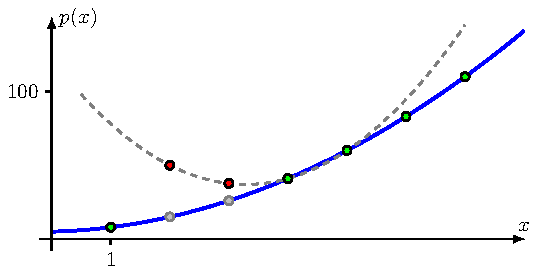
\includegraphics[width=\textwidth]{papers/reedsolomon/figures/polynom2}
    % polynomraw

\newcommand{\teiler}{40}


%//////////////////////////////////////

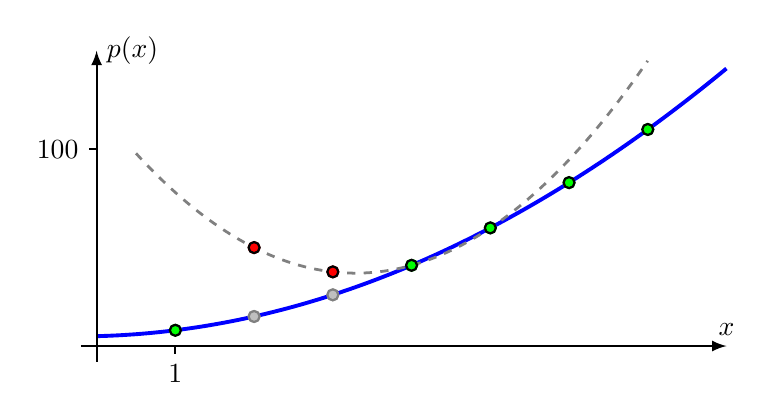
\begin{tikzpicture}[>=latex,thick,]
	\draw[color=blue, line width=1.4pt] 
	plot[domain=0:8, samples=100]
	({\x},{(2*\x^2+1*\x+5)/\teiler});

	\draw[->] (-0.2,0) -- (8,0) coordinate[label={$x$}];
	\draw[->] (0,-0.2) -- (0,150/\teiler) coordinate[label={right:$p(x)$}];
	
	\def\punkt#1{
		\fill[color=green] #1 circle[radius=0.08];
		\draw #1 circle[radius=0.07];
	}

	\def\hellpunkt#1{
		\fill[color=lightgray] #1 circle[radius=0.08];
		\draw[gray] #1 circle[ radius=0.07];
	}
	
	\draw[color=gray,line width=1pt,dashed] 
	plot[domain=0.5:7, samples=100]
	({\x},{(7.832*\x^2-51.5*\x+121.668)/\teiler});


	\punkt{(1,8/\teiler)}
	\hellpunkt{(2,15/\teiler)}
	\hellpunkt{(3,26/\teiler)}
	\punkt{(4,41/\teiler)}
	\punkt{(5,60/\teiler)}
	\punkt{(6,83/\teiler)}
	\punkt{(7,110/\teiler)}
	

	
	\def\erpunkt#1{
		\fill[color=red] #1 circle[radius=0.08];
		\draw #1 circle[radius=0.07];
	}
	\erpunkt{(2,50/\teiler)}
	\erpunkt{(3,37.66/\teiler)}

	\draw(0,100/\teiler) -- (-0.1,100/\teiler) coordinate[label={left:$100$}];
	\draw(1,0) -- (1,-0.1) coordinate[label={below:$1$}];		
\end{tikzpicture}
	\caption{Polynom $p(x)$ von der Gleichung\eqref{reedsolomon:equation1}}
	\label{fig:polynom}
\end{figure}%
\begin{itemize}
    \item[\textit{1 Fehler}:] Bei einem Fehler können konkurrenzierende, aber falsche Polynome zusammen mit zwei originalen Punkten entstehen.
        Dabei können aber maximal drei Punkte auf diesem Konkurrenzpolynom sein.
        Da 6 > 3 ist, haben wir unser originales Polynom gefunden.
    \item[\textit{2 Fehler}:] Bei zwei Fehlern kann ein Fehler mit zwei originalen Punkten ein konkurrenzierendes, aber falsches Polynom bilden.
        Da der zweite \textcolor{red}{Fehler} frei wählbar ist, kann dieser auch auf dem \textcolor{gray}{Konkurrenzpolynom} liegen, wie in der Abbildung \ref{fig:polynom} zu sehen ist.
        Nun haben wir ein \textcolor{blue}{originales Polynom} mit \textcolor{darkgreen}{fünf} übereinstimmenden und ein konkurrenzierendes mit vier Punkten.
        Da fünf noch grösser als vier ist, können wir sagen, welches das Originalpolynom ist.
    \item[\textit{3 Fehler}:] Bei drei kann genau wie bei ein oder zwei Fehlern ein konkurrenzierendes Polynom mit einem Fehler und zwei originalen Punkten bestimmt werden.
        Auch hier sind die anderen Fehler frei wählbar und liegen auf dem Konkurrenzpolynom.
        Nun ist es so, dass fünf Punkte auf diesem konkurrenzierenden Polynom und vier Punkte auf dem originalen liegen.
        Das Originalpolynom kann nicht mehr gefunden werden.
    \item[\textit{4 Fehler}:] Bei vier kann noch erkannt werden, dass Fehler aufgetreten sind, da drei originale Punkte das ursprüngliche Polynom ergeben.
        Somit haben wir mindestens zwei verschiedene Polynome, was bedeutet, dass Fehler entstanden sind.
    \item[\textit{5 Fehler:}] Bei fünf kann mit den zwei originalen Punkten das originale Polynom nicht mehr erkannt werden und 
        somit kann auch keine Aussage mehr gemacht werden, ob Fehler aufgetreten sind oder nicht.
\qedhere
\end{itemize}
\end{beispiel}

\section{Anzahl Übertragungswerte bestimmen
\label{reedsolomon:section:Fehlerkorrekturstellen}}
Um zu bestimmen, wie viele zusätzliche \textcolor{darkgreen}{Übertragungspunkte} notwendig sind, um die Fehler zu korrigieren,
    muss man zuerst wissen, wie viele \textcolor{blue}{Datenwerte} gesendet und wie viele \textcolor{red}{Fehler} erkannt werden sollen. 
Die Anzahl Datenwerte ergibt die Anzahl
\textcolor{blue}{$k$}
Polynomkoeffizienten
und somit den Grad $k-1$ des Polynoms.
Die Bestimmung der Anzahl \textcolor{red}{$t$} der Fehler, welche korrigiert werden können, braucht Redundanz.
Bilden wir verschieden grosse Polynome und untersuchen diese mit unterschiedlich vielen Fehlern, erkennt man allmählich ein Muster.

\begin{table}%[!ht]
    \centering
    \begin{tabular}{ c c | c} 
        \hline
        Nutzlas & Fehler & Übertragen \\
        \hline 
        3 & 2 & 7 Werte eines Polynoms vom Grad 2 \\ 
        4 & 2 & 8 Werte eines Polynoms vom Grad 3 \\
        3 & 3 & 9 Werte eines Polynoms vom Grad 2 \\ 
        \hline
        $k$ & $t$ & $k+2t$ Werte eines Polynoms vom Grad $k-1$ \\ 
        \hline
    \end{tabular}
    \caption{Bestimmung der Anzahl Übertragungspunkte in Abhängigkeit von den Fehlern.}
    \label{tab:fehlerkorrekturstellen}
\end{table}
\par 
Es müssen mehr Punkte auf dem \textcolor{blue}{originalen Polynom} liegen als auf dem konkurrenzierenden.
Somit braucht man für die Übertragung pro \textcolor{red}{Fehler} zwei Übertragungspunkte mehr.
Wie in der Tabelle \ref{tab:fehlerkorrekturstellen} ersichtlich ist ergibt sich die
Anzahl
\begin{equation}
    \textcolor{darkgreen}{u}=
    \textcolor{blue}{k}+2\textcolor{red}{t}.
    \label{reedsolomon:equation2}
\end{equation}
von \textcolor{darkgreen}{Punkten} für die Übertragung.

Ein Nebeneffekt ist, dass auch $2t$ Fehler erkannt werden können, die aber nicht korrigiert werden können.
Um die Polynomkoeffizienten nach der Übertragung zu rekonstruieren, haben wir jedes mal die Polynominterpolationsmethode angewendet.
Diese Polynominterpolation ist leider schwierig zu berechnen und sehr fehleranfällig.
Es wäre daher einfacher, wenn wir eine alternative Vorgehensweise finden könnten. 


